\documentclass{standalone}
%\usepackage{charter}
%\usepackage{fouriernc}
\usepackage[notextcomp]{kpfonts}
\usepackage[defaultsans]{lato}
\usepackage{inconsolata}
\usepackage{tikz}
\usetikzlibrary{angles,quotes}

\begin{document}
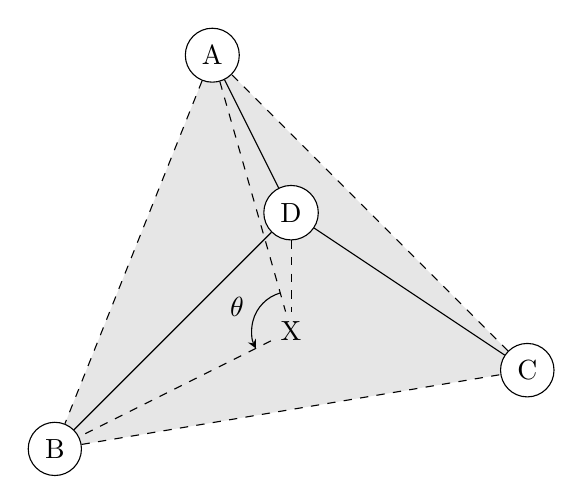
\begin{tikzpicture}


\coordinate (cX) at (0,-1.5);
\coordinate (cD) at (0,0);
\coordinate (cA) at (-1,2);
\coordinate (cB) at (-3,-3);
\coordinate (cC) at (3,-2);

\fill[fill=gray,fill opacity=0.2] (cA) -- (cB) -- (cC);
\node[draw=none]                             (X) at (cX) {X};
\node[circle,draw,fill=white,fill opacity=1] (D) at (cD) {D};
\node[circle,draw,fill=white,fill opacity=1] (A) at (cA) {A};
\node[circle,draw,fill=white,fill opacity=1] (B) at (cB) {B};
\node[circle,draw,fill=white,fill opacity=1] (C) at (cC) {C};

\draw (A) -- (D) -- (B);
\draw (C) -- (D);
\draw[dashed] (D) -- (X);
\draw[dashed] (A) -- (X) -- (B);
\draw[dashed] (A) -- (B) -- (C) -- (A);
\pic[draw,->,>=stealth,"$\theta$",angle eccentricity=1.5] {angle=A--X--B};

\end{tikzpicture}
\end{document}

